\chapter{Implementation}
\label{chap:impl}

The system was implemented by developing new modules and combining both newly-developed components and existing packages together. Most of the codes were written in C/C++, while some of it used python. Server-stubs and client-stubs were employed, and Google's protocol buffer mechanism was used as the way to define the request and response messages shared by the two communicating parties. Open source libraries, such as ZeroMQ and libVLC, were utilized as well. Each module in the system was designed and implemented in an independent, efficient, and extensible way. The rest of this section describes the system implementation in detail.

\section{The Planstep and Emotion Updater: a BayesACT reasoning engine}

We implemented the Planstep- and Emotion- Updater on the basis of the BayesAct program developed by Hoey et al. \cite{hoey2013bayesian}. In their program, a BayesAct framework that models emotional state changes during human interactions was implemented. Based on the framework, this thesis implemented a subclass of class \textit{Agent} that simulates the actions of an automated assistant in a hand-washing scenario. The subclass is called \textit{Assistant}. Class \textit{Assistant} has an attribute field denoting the values of observed behaviours, and has methods that update planstep belief states based on observations. A function to get an estimation of the ``current most-likely planstep'' was defined in \textit{Assistant} as well. The function returns the planstep that has the highest probabilities in the planstep distribution. POMDP observation functions were also defined in \textit{Assistant}. 

Noting the fact that an integer denoting the propositional messages contained in a prompt is used by both the BayesAct and the Prompt-Selector (the numbers come along with a set of predefined video prompts that the selector selects from), consistency between the two encoding systems must be assured. To achieve this, a converter on the server-stub side was implemented. The converter maps propositional descriptions of prompts returned by the server to their corresponding representations used by Prompt-Selector. Since ``turning on water'' and ``turning off water'' are denoted by same integers in BayesAct, additional information such as estimation of the current most-likely planstep is needed for the conversion. The converter is called before the server-stub packs and sends replies back to the client-stub. Relationships between the encoding systems of representing propositions used by BayesAct and the Prompt-Selector are illustrated in Table~\ref{table:prompt-number-def}.

%
% table: Mapping between action suggested in BayesAct and prompt content representations in Prompt-Selector
\begin{table}
\centering
\caption{Mapping between action suggested in BayesAct and prompt content representations in Prompt-Selector}
\label{table:prompt-number-def}
\begin{tabular}{| l | p{5cm} | p{5cm} |}
\hline
Action description & Representation number in BayesAct & Representation number in Prompt-Selector \\ \hline
no prompts needed & 0 & 0\\ \hline
ask the user to put on soap & $1$ & $2$ \\ \hline
ask the user to rinse hands & $3$ & $3$ \\ \hline
ask the user to turn on water & $2$ & $1$ \\ \hline
ask the user to turn off water & $2$ & $4$ \\ \hline
ask the user to to dry hands & $4$ & $5$ \\ \hline
tell the user all has been done & N/A & $6$ \\ \hline
Invalid/undefined prompts & N/A &$-1$ \\ \hline
\end{tabular}
\end{table}

Another minor problem is to choose a proper policy based on which propositional content of a prompt (i.e. what action should the user take) is produced. As far as the propositional content generation policy is concerned, two options are provided by the original program: a POMCP policy and a heuristic policy. The POMCP policy computes a utility function which looks several steps further to produce prompts, while the heuristic policy constructs prompts based on mappings between the estimation of the ``current most-likely  planstep'' and system actions. The mappings in the heuristic policy are obtained by heuristic knowledge and are shown in Table~\ref{table:heuristic-policy}. Considering the fact that the heuristic policy runs faster and is sufficient for our prototype system, which is used to demonstrate the feasibility of including emotional intelligence in a practical system, the heuristic policy was chosen in our approach.

%
% table: Action suggestions basing on the current most-likely planstep (heuristic policy)
\begin{table}
\centering
\caption{Action suggestions basing on the current most-likely planstep (heuristic policy)}
\label{table:heuristic-policy}
\begin{tabular}{| l | l | l | l | l |}
\hline
\multicolumn{4}{|c|}{Current Most-likely Planstep} & \multirow{2}{*}{ Actions Suggested} \\ \cline{1-4} 
Number & Soap(dirty/soapy/clean) & Water(on/off) & Hand(wet/dry) & \\ \hline
0 & dirty & off & dry & turn on water \\ \hline
1 & dirty & on & dry & put on some soap \\ \hline
2 & soapy & off & dry & turn on water \\ \hline
3 & soapy & on & dry & rinse hands \\ \hline
4 & clean & on & wet & turn off water \\ \hline
5 & clean & off & wet & use towel \\ \hline
6 & clean & on & dry & turn off water \\ \hline
7 & clean & off & dry & N/A \\ \hline
\end{tabular}
\end{table}

As discussed in the previous chapter, BayesAct is treated as a server in our implementation. Both a server-stub and a client-stub are developed. The server-stub listens to client requests at all times, and if there are any, processes them. The request processing tasks include: decoding the requests, passing arguments encoded in the request to the server for it to update belief states, and packing and replying the prompt descriptions obtained from the server to the client-stub. The client-stub packs and sends user hand-actions and EPA values of these actions to the server-stub, and waits for replies. When a reply is received, the client-stub decodes it, and converts the information accordingly, e.g. passes the information to a Prompt-Selector, where appropriate video prompts are selected.

\begin{verbatim}

message BayesactRequest {
  required double evaluation = 1 [default = 0.0];
  required double potency = 2 [default = 0.0];
  required double activity = 3 [default = 0.0];
  required int32 hand_action = 4 [default = -1];
 }
 
 message BayesactResponse {
  required double evaluation = 1 [default = 0.0];
  required double potency = 2 [default = 0.0];
  required double activity = 3 [default = 0.0];
  required int32 prompt = 4 [default = -1]; // propositional representation  
  required bool is_done = 5 [default = false]; // if reaches the last planstep
 }

\end{verbatim}

Definitions of request and response messages shared between the two communicating parties are defined using Google's protocol buffers (shown above), and the stubs are implemented using zmq libraries \footnote{The official website of the zmq library: \url{http://zeromq.org/}.}. The stubs bind or connect to given addresses in their constructors, and with the help of zmq, they are able to easily send and receive messages to/from each other. Among all the benefits that using protocol buffers and zmq brings us, the language-neutral advantage is one that is worthy of particular attention: it allows us to combine easily the BayesAct server and its stub with all other components together as a whole system, where the former ones were implemented in python, while the latter ones were implemented using C/C++.


\section{The EPA-Calculator and the Buffer: computing and temporally smoothing EPA's}

Hands' coordinates obtained from the hand-tracker server are fed into an EPA-Calculator, which represents user behaviours as EPA values. In our prototypical approach, the \textit{Evaluation} (or the ``E'' value) of the user's behaviour in all situations are computed as a neutral value and is considered as an uninformative observation in the Emotion Updater. The \textit{Potency} (or the ``P'' value) and \textit{Activity} (or the ``A'' value) are computed in the EPA-Calculator based on the distances between the user's two hands within a same frame and the distances that the user's hands have moved between neighbouring frames, respectively. The E, P, and A values computed for user behaviours in the EPA-Calculator are temporally smoothed in the Buffer before fed into the Planstep and Emotion Updater.

A parameter $n$ is used to compute the $P$ and $A$ values of the user's behaviour. The average distance between the user's two hands in a set of $n$ neighbouring frame is scaled to the $P$ value of the user's behaviour in the EPA-Calculator. The average distance $Dist[i]$ of frames $i-n+1, i-n+2, ... , i$ can be computed using the following formula:
$$Dist[i]=\dfrac{1}{n} \sum_{k=i-n+1}^{i}dist(positions[k,0],positions[k,1])$$
where function $dist: Point \times Point \to real\ number$ computes the distance between two points, and $positions[k,0]$ and $positions[k,1]$ are the coordinates of the user's left/right hand in frame $k$. A piecewise linear interpolation method is used to map the average distance $Dist[i]$ to the $P[i]$, which is the $P$ value of the user's behaviour at frame $i$. Two same-length ascendingly sorted arrays of thresholds, $potency$ and $distance$, are defined. The first and the last elements of array $potency$ are $-4.3$ and $4.3$, respectively. And the first and last elements of array $distance$ are $-$ and $+$, respectively. The algorithm used in the mapping between $Dist[i]$ and the $P[i]$ is as following:
$$P[i]=(Dist[i]-distance[k-1]) * \dfrac{potency[k]-potency[k-1]}{distance[k]-distance[k-1]} + potency[k-1]$$
where $distance[k] \geq Dist[i]>distance[k-1]$.

Finally, a set of $P$ values, say from $P[i]$ to $P[j]$, $i \leq j$, are temporally smoothed in the Buffer as the final $P$ value that is fed into the Emotion Updater. The smoothing algorithm ensures that the influence of the $P[k], i \leq k \leq j$, decays with time. The smoothing algorithm used in the Buffer can be illustrated by the following formula:
$$P=\sum_{k=i}^{k=j}(\dfrac{alpha}{alpha+1})^{j-k}*\dfrac{1}{alpha+1}*P[k]$$ where $alpha \geq 0$.
If $alpha=0$, then $P=P[j]$, which means that no temporal smoothing is used to compute the final $P$ value.

Similarly, the $A$ value of the user's behaviour are calculated based on the average of the distances his/her hands move between $n$ neighbouring frames. The average movement $Diff[i]$ during frames $i-n+1, i-n+2, ... , i$ can be computed by the following formula:
$$Diff[i]=\dfrac{1}{n-1}\sum_{k=i-n+2}^{i}maxDiff(positions[k],positions[k-1])$$
where $position[k]$ contains a pair of coordinates representing the user's left and right hand locations respectively in frame $k$, and function $maxDiff: (Point_a, Point_b) \times pair(Point_c, Point_d) \to real\ number$ returns $max(dist(Point_a, Point_c), dist(Point_c, Point_d))$. Piecewise linear interpolation method is used to map the average distance $Diff[i]$ to the $A[i]$, which is the $A$ value of the user's behaviour at frame $i$. Two same-length ascendingly sorted arrays of thresholds, $activity$ and $difference$, are defined. The first and the last elements of array $activity$ are $-4.3$ and $4.3$, respectively. And the first and last elements of array $difference$ are $-$ and $+$, respectively. The mapping algorithm between $Diff[i]$ and $A[i]$ is as following:
$$A[i]=(Diff[i]-difference[k-1])*\dfrac{activity[k] - activity[k-1]}{difference[k] - difference[k-1]}+activity[k-1]$$
where $difference [k] \geq Diff[i] > difference[k-1]$.

Finally, a set of $A$ values, say from $A[i]$ to $A[j]$, $i \leq j$, are temporally smoothed in the Buffer as the final $A$ value that is fed into the Emotion Updater. The smoothing algorithm ensures that the influence of the $A[k]$, $i \leq k \leq j$, decays with time. The smoothing algorithm used in the Buffer can be illustrated by the following formula:
$$A=\sum_{k=i}{k=j}(\dfrac{alpha}{alpha+1})^{j-k}*\dfrac{1}{alpha+1}*A[k]$$ where $alpha \geq 0$.
If $alpha=0$, then $A=A[j]$, which means that no temporal smoothing is used to compute the final $A$ value.

Note that in the computations of $P$ and $A$, variables $n$, $potency$, $distance$, $activity$ and $difference$ are used in the EPA-Calculator and $alpha$ is used in the Buffer. The values of these variables need to be set when running the system. Chapter~\ref{chap:result} described a way to set the thresholds $potency$, $distance$, $activity$ and difference by statistical results from experiments. In this prototypical approach, the unweighted means of distances were used and scaled to $P$'s and $A$'s; weighted average, and/or more other features can be included as indicators for the EPA values of user behaviours in future approaches.

\section{The Observer: an extension to existing hand-tracker}

Similar to the Planstep and Emotion Updater, we implemented the Observer as an extension, with a server-stub and client-stub added and several changes made to parameter values and other details, to the tracker Czarnuch developed \cite{czarnuch2014}. We explain in the following paragraphs the algorithms used in Czarnuch's tracker, the changes we made to the original program, and the implementation details of the server and client stubs. Note that a kinect camera is mounted above the sink when the Observer is in use.

In the original program, decision trees were trained on a set of images that were manually annotated to optimize key parameters. The trained tracker is then used to classify body parts in depth images grabbed from an overhead perspective. The tracker first generates a random decision forest using a simple depth feature to provide intermediate multiclass probability density functions (PDF) for each sampled image pixel. It then proposes final body part positions by aggregating the information contained in the underlying PDF. As explained by Czarnuch \cite{czarnuch2014}, the pre-trained decision trees included in their original program are able to classify body parts (including head and hands) as long as the camera is mounted from an overhead perspective to the objects and areas of interest. 

After body parts (e.g. hands) are classified, the original tracker uses a location-based method to identify ``hand behaviours''. It first checks which pre-defined areas the user's hands are currently inside of. If multiple areas are detected, then a set of rules, such as comparing the distances from the areas' centers and current hand-locations, are applied to decide the ``winner'' area that user's hands fall in at the moment. For example, suppose a ``soap area'' is defined as $(s_{x}, s_{y}, s_{z}, s_{r})$, where $(s_{x}, s_{y}, s_{z})$ are the coordinates of the area center in world space and $s_{r}$ represents the radius of this area (i.e. the area is defined as within a spherical surface). If the current left hand-location is detected as at point $(l_{x}, l_{y}, l_{z})$, where $(l_{x}-s_{x})^{2} + (l_{y}-s_{y})^{2} + (l_{z}-s_{z})^{2} \leqslant s_{r}^{2}$, then this left hand is considered to overlap with the ``soap area'', which implies an behaviour of ``using the soap''. If the user's left hand overlaps with multiple areas, then the one with a closer center to the hand's location becomes the winning area. This same ``detection of area and behaviour'' process is performed for both of the user's hands and for all pre-defined areas. Note that in this approach, the user's two hands can be detected as performing different behaviours at the same time - one using the soap within the ``soap area'' and the other one doing nothing in particular at the sink. In the Observer we developed, when different areas/behaviours are detected for the user's two hands, a function comparing the two and returning a single winning area/action is called. More details about this comparison function are explained in the following paragraphs.

%
%figure: Screenshot of Czarnuch's tracker recognizing user's head and hands
\begin{figure}[htb]
\centering
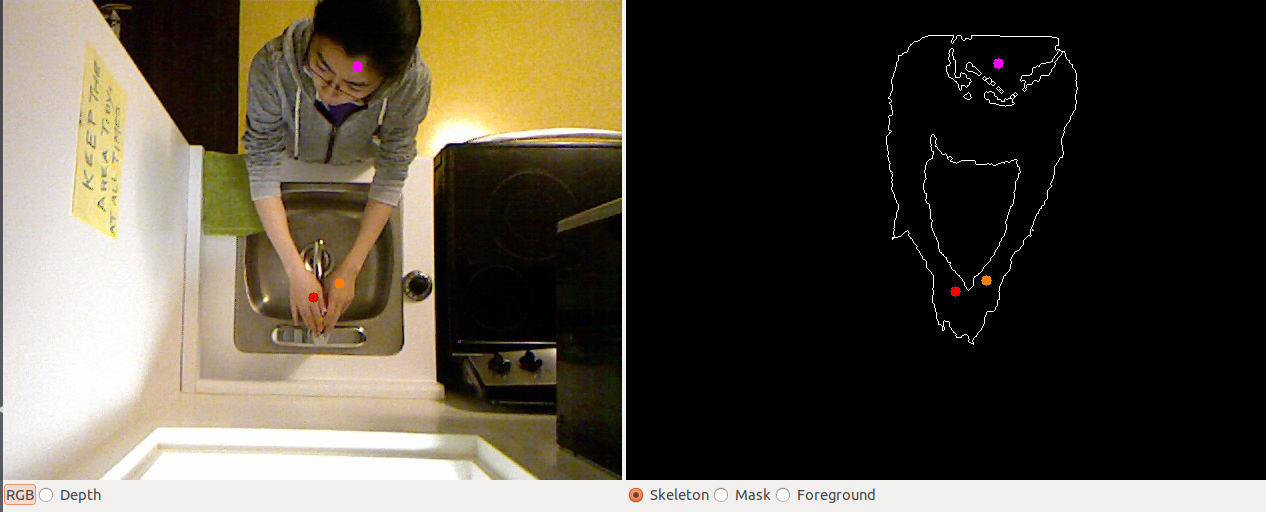
\includegraphics[width=0.9\linewidth]{fig/handtracker-performance.png}
\caption{Screenshot of Czarnuch's tracker recognizing user's head and hands}
\label{fig:handtracker-performance}
\end{figure}

Figure~\ref{fig:handtracker-performance} shows that the original tracker can recognize and return hand-positions with enough accuracy in our application scenario. Having this result, we did not retrain the model in our approach. However, if researchers were to retry our experiments, or to use Czarnuch's program in their own applications, they might need to recollect data and retrain the model. Luckily, Czarnuch included both data collection and data training modes in his program.

In our Observer, the positions and coverages of the interested areas are assigned in a configuration file. To be specific, coordinates and radiuses of seven areas, including AWAY, SINK, SOAP, WATER, Left\_TAP, Right\_TAP, TOWEL are defined. Priority levels to user behaviours are defined as well (see Table~\ref{table:area-action}). In the Observer, when different areas/behaviours are detected for the user's two hands, a function comparing the priority levels of two and returning the one with higher priority is called. Moreover, noticing that both the Observer and the Planstep and Emotion Updater represent areas/actions by integers, we implemented a converter function to convert between the two encoding systems to ensure that the two encoding systems are consistent with each other. Table~\ref{table:area-action} gives an overview of the relationships between areas and the user behaviours implied by them, along with the priority levels assigned to and the representations numbers used for these areas.

%
% table: Relationships between areas and the actions implied
\begin{table}
\centering
\caption{Relationships between areas and the actions implied}
\label{table:area-action}
\begin{tabular}{| l | l | p{2cm} | p{3cm} | p{3cm} |}
\hline
Area Name & Action Implied & Priority Level & 
Representation Number used in the Observer  & Representation Number used in the Updater \\ \hline
N/A & undefined action & $0$ & $0$ & $0$ \\ \hline
AWAY & doing nothing & $1$ & $1$ & $0$ \\ \hline
SINK & doing nothing & $2$ & $2$ & $0$ \\ \hline
SOAP & putting on soap & $6$ & $3$ & $1$ \\ \hline
WATER & rinsing hands & $4$ & $5$ & $3$ \\ \hline
Left\_TAP & turning on/off water & $5$ & $4$ & $2$ \\ \hline
Right\_TAP & turning on/off water & $5$ & $4$ & $2$ \\ \hline
TOWEL & drying hands & $3$ & $6$ & $4$ \\ \hline
\end{tabular}
\end{table}

As discussed previously, the Observer is treated as an observation server in our implementation. Both a server-stub and a client-stub were developed. The server-stub listens to client requests at all times, and if there are any, processes them, which includes decoding the requests, asking the server for current hand-coordinates and hand-actions, and packing and replying to the client-stub the answers. The client-stub sends requests (for current user behaviours and hand locations) to the server-stub, and waits for replies. When a reply is received, the client-stub decodes it, and converts the information accordingly (e.g. maps the representation numbers of hand-actions used by the hand-tracker to the ones used by BayesAct).

Definitions of request and response messages should be shared between the two communicating parties. With the benefit of language-neutral, platform-neutral, and easily extendable, Google's protocol buffers were used to define the message structures (shown below).

\begin{verbatim}
message HandTrackerRequest {
  optional int32 timestamp = 1 [default = -1]; // -1 means this field is not used
}

message HandTrackerResponse {
  message HandPosition {
    required float x = 1 [default = 0.0];
    required float y = 2 [default = 0.0];
    required float z = 3 [default = 0.0];
  }
  required HandPosition left_hand_position = 1;
  required HandPosition right_hand_position = 2;
  required int32 action = 3 [default = 0];
  optional int32 timestamp = 4 [default = -1];
}
\end{verbatim}

The server-stub and client-stub can be easily implemented using zmq libraries. The stubs only need to bind or connect to given addresses in their constructors, and with the help of zmq, they are able to easily send and receive messages to each other. Of course, encoding and decoding of messages should be processed according to the message definitions above before sending out and after receiving messages, respectively. The client-stub also needs to map the representation numbers of hand-actions used by the hand-tracker to the ones used by BayesAct after decoding messages.

A function called processRequestsIdle() is implemented on the server side to have the server-stub listen to client-stub requests at all times. It checks the existence of requests, and processes them accordingly if needed. The function, along with another function called handTrackerIdle(), which observes and returns hand-locations and hand-actions, are registered as the server's idle callbacks.


\section{The Output Part: Prompt Selector and Player}

Both propositional and emotional prompt descriptions are passed into a Prompt Selector, where a most appropriate video prompt is selected from a set of pre- generated and rated prompts. After this final prompt is selected, it will be sent to a Prompt Player, which was implemented by us using VLC SDK, for display. This sub-section illustrates the implementation details of the Prompt Selector and Player in order.

The set of pre-generated and rated video prompts in Malhotra's survey \cite{malhotra2014} serves as the prompt dataset for our Prompt Selector. Figure~\ref{fig:sample-prompt} with the two screenshots of prompts instructing the user to use some soap gives a general idea of what the video clips look like. Note that the message contents of the two prompts are the same (i.e. they intend to instruct the user to do same actions); it is the way how these messages were expressed that differ them apart. The character in the first screenshot was suggesting the user to ``try putting on some soap'' with widely-open hands and a kind smiling face, giving us the impression of a nice, a little bit dominant and active lady. On the contrary, the character in the second screenshot was stating ``If you want to put on some soap, there is a soap pump lying around.'' with her hands crossed and her face unhappy. Different from the first one, the second character gives us the impression of uncaring and passive. In fact, the survey results align with our intuitive impressions: the first video prompt was rated $[1.56, 1.17, 1.35]$ for its EPA values by participants, while the second one got a rate of  $[-0.94, -0.67, 0]$ as its EPA values in the same survey.


%
%figure: Screenshots of two video prompts stating same propositional messages
\begin{figure}[htb]
\centering
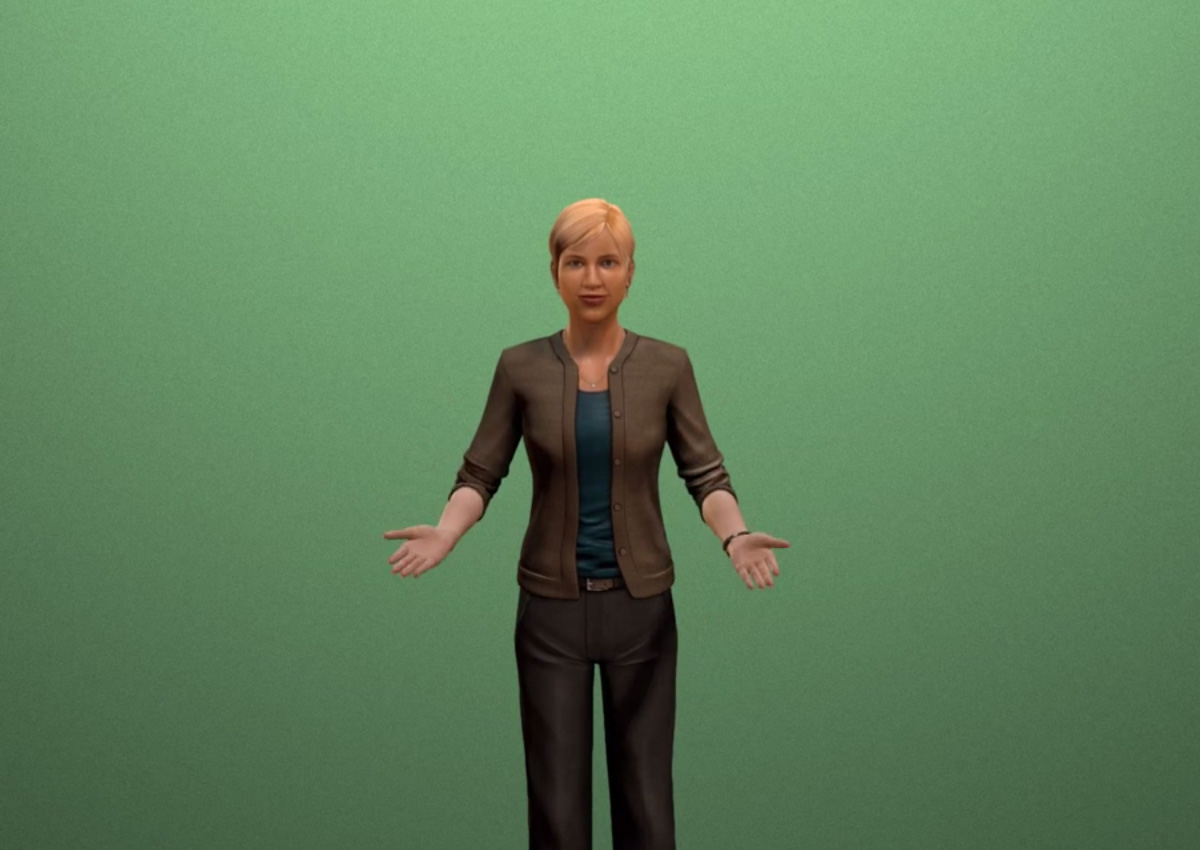
\includegraphics[width=0.45\linewidth]{fig/prompt1.jpg}
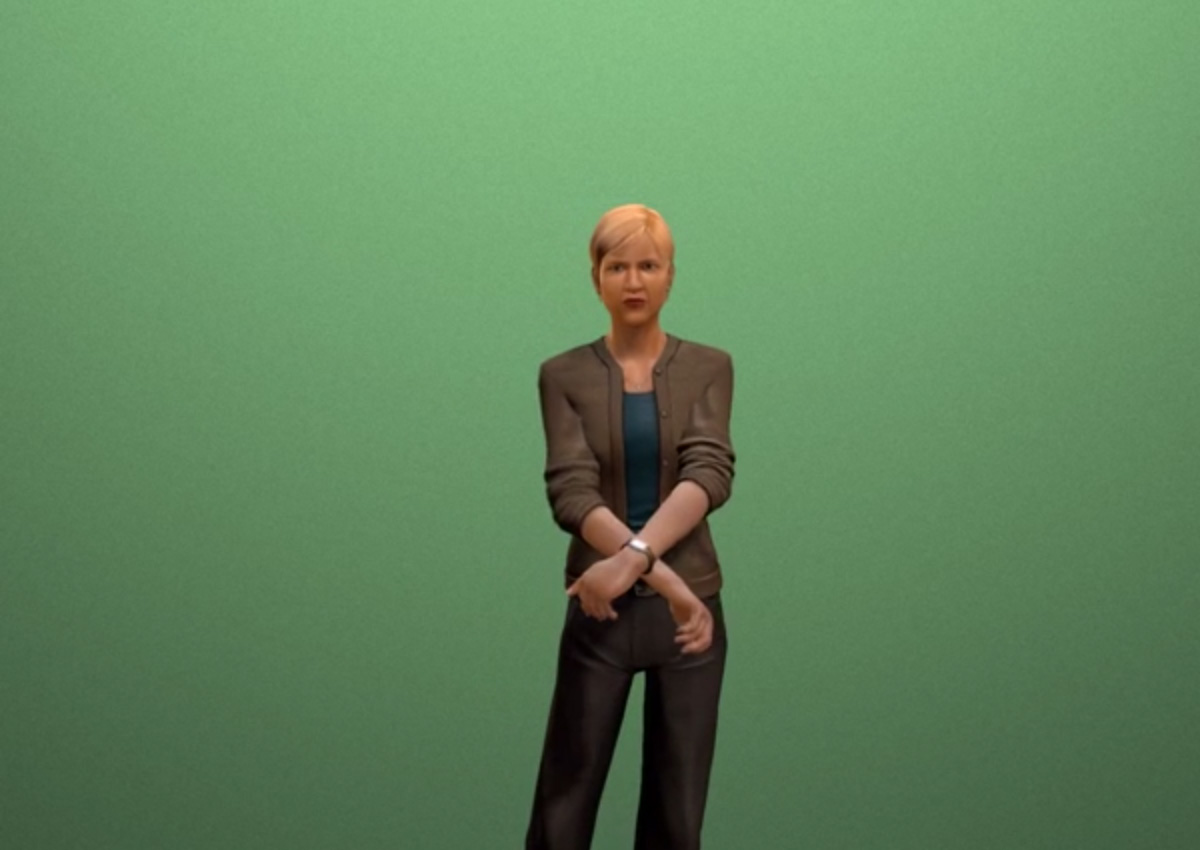
\includegraphics[width=0.45\linewidth]{fig/prompt2.jpg}
\caption{Screenshots of two video prompts stating same propositional messages}
\label{fig:sample-prompt}
\end{figure}

Each of the prompts in the dataset of the Prompt Selector has two labels: one states the propositional content of the prompt while the other one describes it emotionally. The propositional labels are assigned according to the intent of the prompts and are represented by integers. The mappings from ``intent of prompts'' to ``propositional labels'' are stated in Table~\ref{table:prompt-number-def}. The emotional labels, on the other hand, are defined as the EPA values participants rated in the survey. For example, the prompt from which the first screenshot is labelled as $[1.56, 1.17, 1.35]$ for its emotional annotation.

Given the propositional and emotional descriptions of desired prompts (obtained from the BayesAct server component), the Prompt Selector is able to select the most proper prompts in the dataset via a distance-based method. To illustrate how the selector works, we first define the distance between two vectors of EPA values as the weighted Euclidean distance between them: \newline
$dist((E_1, P_1, A_1), (E_2, P_2, A_2))=\sqrt{(w_E(E_1-E_2))^2+(w_P(P_1-P_2))^2+(wA(A1-A2))^2}$,
where $w_E$, $w_P$ and $w_A$ are weights for the three dimensions respectively. We then define the emotional distance between two prompts as the distance between their emotional annotations, i.e. the EPA values assigned to them. When given the propositional and emotional descriptions of the desired prompt, the selector selects out the video prompt that simultaneously has the same propositional label as and the minimal emotional distance to that desired prompt. In our implementation, the weights $w_E$, $w_P$ and $w_A$ are assigned values $\{1, 1, 1\}$; other values and even other definitions of the distances can be tried out in future improvements.

After the proper prompt is selected, a Prompt Player is used to display the video prompt. The Prompt Player was implemented using libVLC (VLC SDK), a mature and easy-to-use media framework that can be embedded into systems to provide multimedia capabilities for the applications.



